\documentclass[12pt]{article}
\input{preamble}

\pagestyle{fancy}
\fancyhf{}

\rhead{Nørre Gymnasium\\
2.c
}


%Husk at rette modul og dato!
\lhead{Matematik B\\
Aflevering 6
}
\chead{20/4/2022
}

\cfoot{Side \thepage \hspace{1pt} af \pageref{LastPage}}

\begin{document}

%Udfyld afsnit herunder og lav til egen Latex-fil

%Kopier følgende til overskrift:

%\begin{center}
%\Huge
%Aflevering 1
%\end{center}
%\section*{Opgave 1 \large (med hjælpemidler)}
%\stepcounter{section}
%Overskrift
\begin{center}
\Huge
Aflevering 6
\end{center}

\section*{Opgave 1 (uden hjælpemidler)}
\stepcounter{section}

En linje $l$ er givet ved ligningen 
\begin{align*}
-10(x+7) + 5(y-8) = 0
\end{align*}
\begin{enumerate}[label=\roman*)]
\item Bestem en normalvektor til $l$.
\item Bestem et punkt, $l$ går gennem. 
\end{enumerate}


\section*{Opgave 2 (uden hjælpemidler)}

Af Fig. \ref{fig:poly} ser vi parablen for et andengradspolynomium $f$ givet ved
\begin{align*}
f(x)=ax^2+bx+c. 
\end{align*}

\begin{figure}[H]
\centering
\begin{tikzpicture}
\begin{axis}[axis lines = middle, ticks = none, xmin = -2, xmax = 2, ymin = -3, ymax = 3]
\addplot[color = blue!50, samples = 1000] {-x^2+x+1};
\end{axis}
\end{tikzpicture}
\caption{Grafen for polynomiet $f$}
\label{fig:poly}
\end{figure}

\begin{enumerate}[label=\roman*)]
\item Bestem fortegnet for koefficienterne $a$, $b$ og $c$. Begrund dit svar.
\item Bestem fortegnet for diskriminanten $d$. Begrund dit svar.
\end{enumerate}

\section*{Opgave 3 (uden hjælpemidler)}

En producent af en automatisk udstener til oliven lover at 99$\%$ af alle oliven bliver korrekt udstenet. En olivenbonde udstener 100.000 oliven med denne olivenudstener. 

I en model angiver den binomialfordelte stokastiske variabel $X$ antallet af oliven, der bliver korrekt udstenet hos olivenbonden.
\begin{enumerate}[label=\roman*)]
\item Bestem middelværdien for $X$. 
\end{enumerate}

\section*{Opgave 4 (uden hjælpemidler)}

Et tredjegradspolynomium $f$ er givet ved
\begin{align*}
f(x) = x^3-2x+4.
\end{align*}
\begin{enumerate}[label=\roman*)]
\item Bestem $f(-3)$.
\item Bestem $f'(x)$.
\item Bestem $f'(2)$, og forklar hvad dette betyder for hældningen af grafen for $f$ i punktet $(2,f(2))$. 
\end{enumerate}


\section*{Opgave 5 (uden hjælpemidler)}
Af Fig. \ref{fig:topoly} ses graferne for en funktion $f$ og dens differentierede $f'$. 
\begin{figure}[H]
\centering
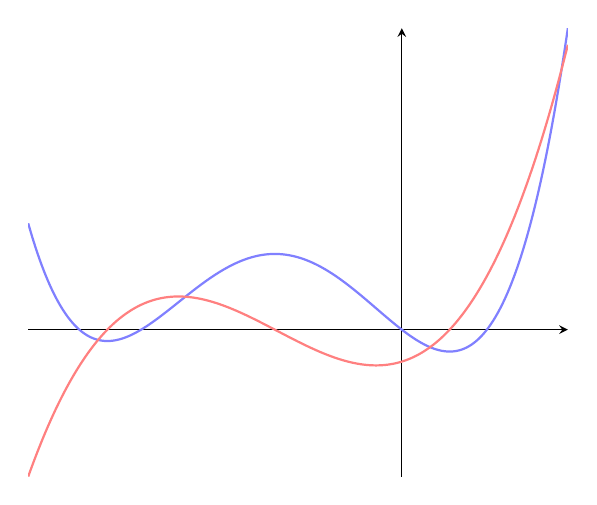
\begin{tikzpicture}
\begin{axis}[axis lines = middle, ticks = none,xmin = -9,xmax = 4]
\addplot[color = blue!50, thick, samples = 1000, domain = -9:4] {x^4 + 12* x^3 + 20 *x^2 - 100*x};
\addplot[color = red!50, thick, samples = 1000, domain = -9:4] {4*x^3 + 36* x^2 + 40*x - 100};
\end{axis}
\end{tikzpicture}
\caption{Grafer for $f$ og $f'$}
\label{fig:topoly}
\end{figure}

\section*{Opgave 6 (med hjælpemidler)}


I en by er luftpartikelkoncentrationen af en bestemt type udstødningspartikel målt fra år $2000$ til år $2010$. Den målte koncentration (i ppm) som funktion af tiden (i år) kan ses af følgende tabel:
\begin{center}
\begin{tabular}{c|c|c|c|c|c|c|c|c|c|c|c}
$t$  & 0 & 1 & 2 & 3 & 4 & 5 & 6 & 7 & 8 & 9  \\
\hline
$C$  &11.67 & 35.15 & 42.49 & 68.97 & 55.61 & 92.73 & 103.22 & 150.53 & 185.23 & 244.42
\end{tabular}
\end{center}

\begin{enumerate}[label=\roman*)]
\item Vi antager, at sammenhængen mellem tiden $t$ og koncentrationen $C$ er på formen
\begin{align}\label{eq:lin}
C(t) = at+b.
\end{align}
Bestem $a$ og $b$, så denne sammenhæng passer bedst på punkterne. 
\item Lav residualanalyse på denne model og vurdér, om en sammenhængen af typen \eqref{eq:lin} beskriver datasættet godt.
\item En genovervejelse af kilden til denne forurening får os til at tro, at sammenhængen mellem luftpartikelkoncentrationen og tiden er givet ved en eksponentiel sammenhæng i stedet. Lav eksponentiel regression på datasættet og kommentér på resultatet.
\item Lav residualanalyse på den eksponentielle model og sammenlign med den tidligere model. Hvilken model virker til at være mest valid?
\item Bestem residualet for begge modeller i år $2005$.
\end{enumerate}

\section*{Opgave 7 (med hjælpemidler)}

Et polynomium $f$ er givet ved
\begin{align*}
f(x) = x^5-10x^2+3x-10.
\end{align*}
\begin{enumerate}[label=\roman*)]
\item Tegn grafen for $f$. 
\item Løs ligningen $f'(x) = 0$.
\item Bestem monotoniforholdene for $f$. 
\end{enumerate}


\section*{Opgave 8 (med hjælpemidler)}
En cirkel $c$ er givet ved ligningen 
\begin{align*}
x^2-4x+y^2+4y = 17
\end{align*}
\begin{enumerate}[label=\roman*)]
\item Angiv centrum og radius for cirklen $c$ ved at omskrive den til formen
\begin{align*}
(x-a)^2+(y-b)^2 = r^2
\end{align*}
\end{enumerate}
Punktet $P = (3,2)$ ligger på $c$. 
\begin{enumerate}[label=\roman*)]
\stepcounter{enumi}
\item Bestem en ligning for tangenten til cirklen $c$ i punktet $P$.
\end{enumerate}

\section*{Opgave 9 (med hjælpemidler)}
I et stort glas med oliven tæller vi antallet af oliven til at være 120. Vi observerer, at der er sten i $8\%$ af olivenene i glasset. 
\begin{enumerate}[label=\roman*)]
\item Bestem et $95\%$ konfidensinterval for andelen af oliven i denne type glas af oliven. 
\end{enumerate}
Vi køber et andet mærke af oliven. I dette observerer vi, at der er sten i $5.8\%$ af olivenene. 
\begin{enumerate}[label=\roman*)]
\stepcounter{enumi}
\item Benyt dit konfidensinterval for at bestemme, om der er signifikant forskel på andelen af sten i glassene med oliven for de to forskellige mærker. 
\end{enumerate} 
\end{document}


